% this file is called up by thesis.tex
% content in this file will be fed into the main document

%: ----------------------- name of chapter  -------------------------
\chapter{Case Studies} % top level followed by section, subsection


Typing on a smartphone is made easier to the user by including auto-correct, but the same tool can not be used for authentication process. Therefore users are left with the task to hit every key accurately or repeat the task until they get it right. 

In this chapter we present the results from a survey made to determine, whether the proposed authentication method increases the user experience.


%: ----------------------- paths to graphics ------------------------

% change according to folder and file names
\ifpdf
    \graphicspath{{X/figures/PNG/}{X/figures/PDF/}{X/figures/}}
\else
    \graphicspath{{X/figures/EPS/}{X/figures/}}
\fi

%: ----------------------- contents from here ------------------------

\section{Validation}
In order to validate the hypothesis, the proposed solution is compared to the conventional ''input credentials'' method in terms of simplicity and user experience. A use case based on social media sign-in was developed. The application is primitive to only test the authentication process. 

In the validation, a tablet LG G Pad 8.3 \footnote[16]{http://www.gsmarena.com/lg\_g\_pad\_8\_3-5673.php} was used. It has a 8.3 inch screen with the resolution of 1200x1920 pixels and is running Android 4.4.2, otherwise called as KitKat \footnote[17]{https://www.android.com/versions/kit-kat-4-4/}.

\subsection{Experimental Setup}
	
In the first application, only the conventional method is used as shown in Figure 5.1. The second application uses the proposed solution, which is divided into two parts: registering an account and authenticating with the stored account. Screenshots of the credentials saving process are seen in Figure 5.2. Once the library is integrated within the app, a button \textit{Save/Get Credentials} appears (1). With the username and password filled in, pressing the mentioned button, the user is requested to validate his password by typing it for the second time (2). Pressing the button \textit{Create}, the user can introduce a pattern (3), after drawing it twice, the process of credentials registration is complete and the user is taken to a list of accounts already stored (4). Screenshots of the authentication sequence are seen in Figure 5.3. The second step of authentication will either start from where registration ended or from a newly opened applications empty main page (1). Pressing the \textit{Save/Get Credentials} button, a list of stored accounts is presented to the user (2). Selecting an account in the list, the user is prompted to draw a pattern (3) and on a successful authentication the user is taken back to the main page with the username and password filled in (4).

To compare these two methods, a questionnaire was composed |Appendix A|. It consists of 10 questions, first 2 are general questions about participants satisfactory to authentication process today. The next two sections, questions 3-6 and 7-10, are more specific to the authentication methods implied to applications used in this case study. 

\subsection{Methodology}
There were 20 participants between the ages of 20 and 30, all day-to-day smartphone users. None of them have expertise in computer science, hence they are only end users. They were asked to first answer the first two questions, then they would perform authentication on the application with the conventional method and respond to question 3-6. Then they would register an account and authenticate themselves with the second application, also change the stored password or pattern and answer the last four questions. 

\begin{figure}[H]
\centering
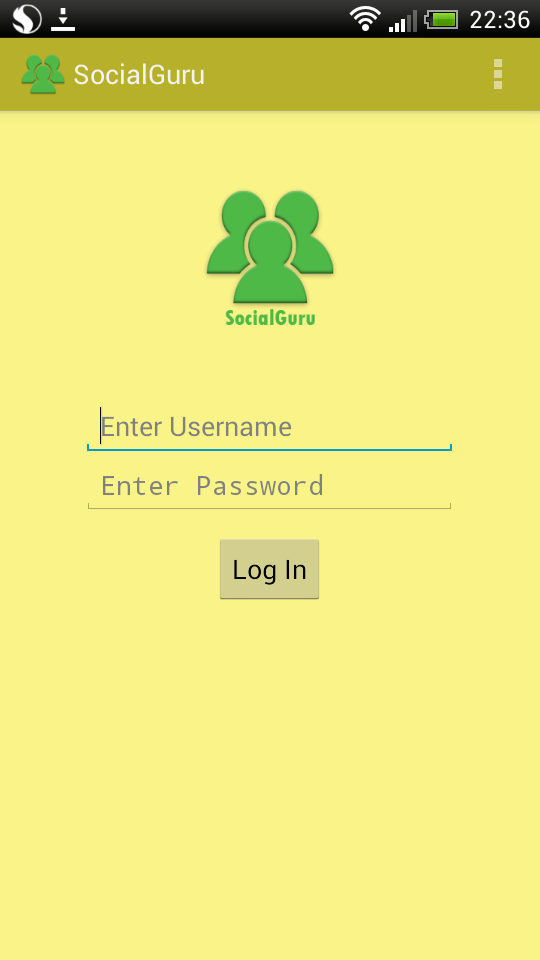
\includegraphics[scale=0.3]{images/nolibrary.png}
\caption{Application with only conventional method.}
\label{fig:nolibrary}
\end{figure}

\begin{figure}[H]
\begin{center}
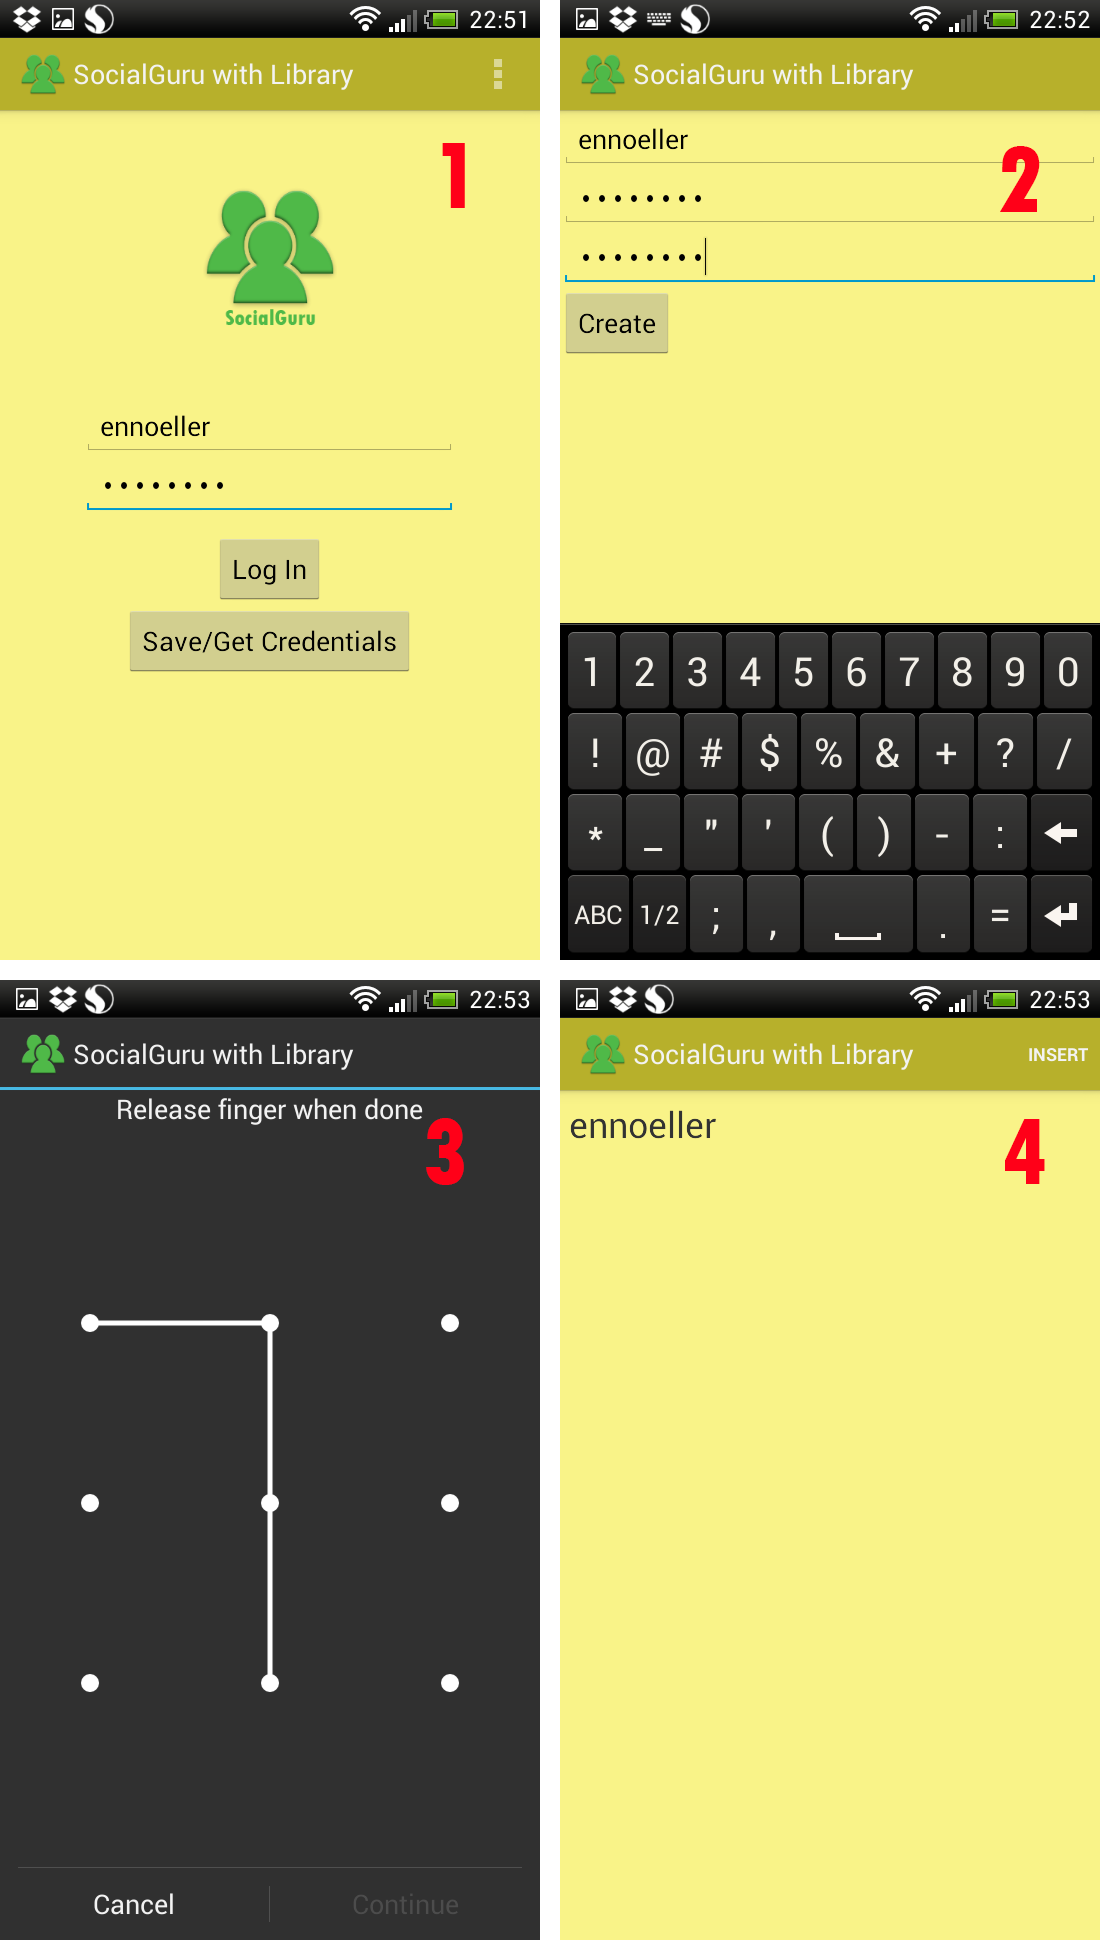
\includegraphics[scale=0.3]{images/reg.png}
\caption{Credentials saving process with the library.}
\label{fig:credentials saving}
\end{center}
\end{figure}

\begin{figure}[H]
\begin{center}
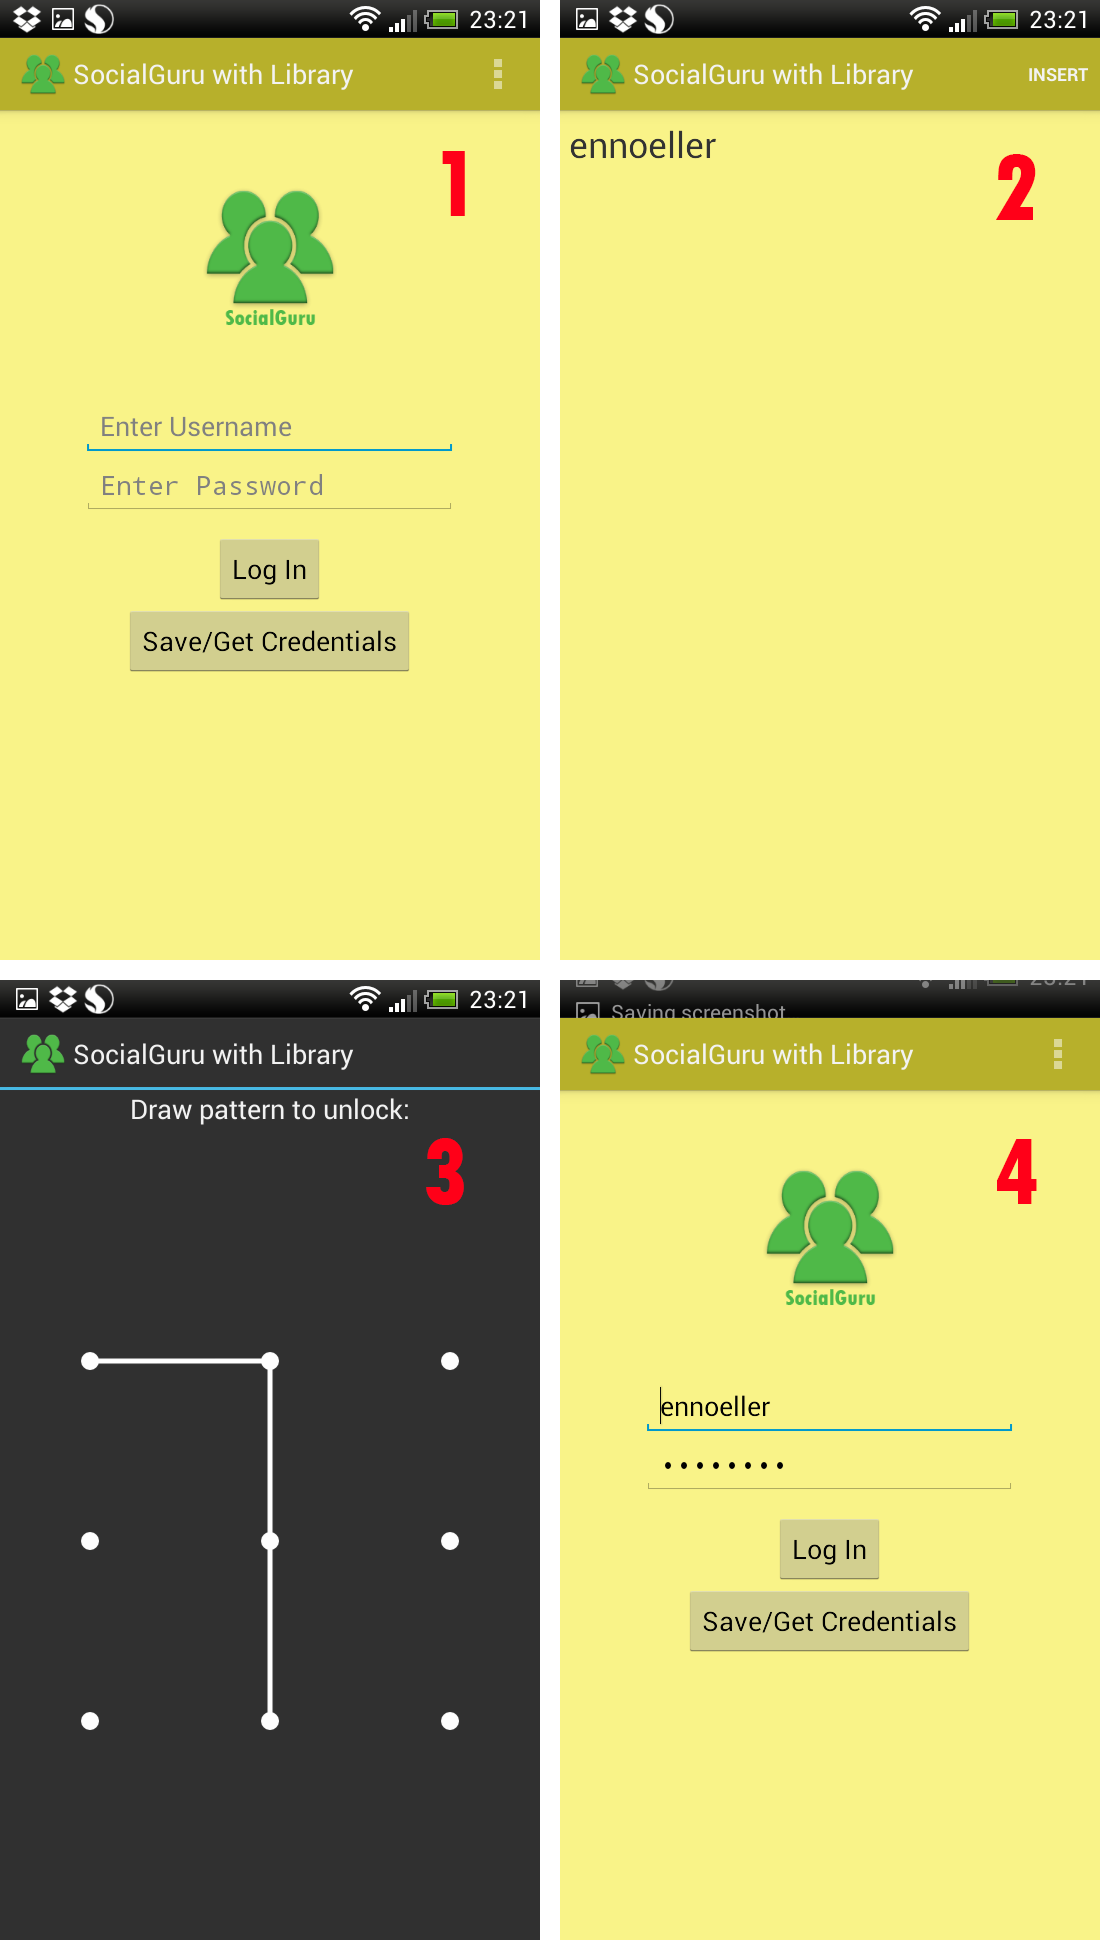
\includegraphics[scale=0.3]{images/auth.png}
\caption{Athentication process with the library.}
\label{fig:authentication}
\end{center}
\end{figure}

\section{Results}

First two questions were about participants opinions about authentication methods used in applications. 65\% of them, shown in Figure 5.4, find that applications do use suitable login methods. 5 out of 7 participants, who find applications not to use suitable methods, brought out that the process should include less typing. 

\begin{figure}[H]
\centering
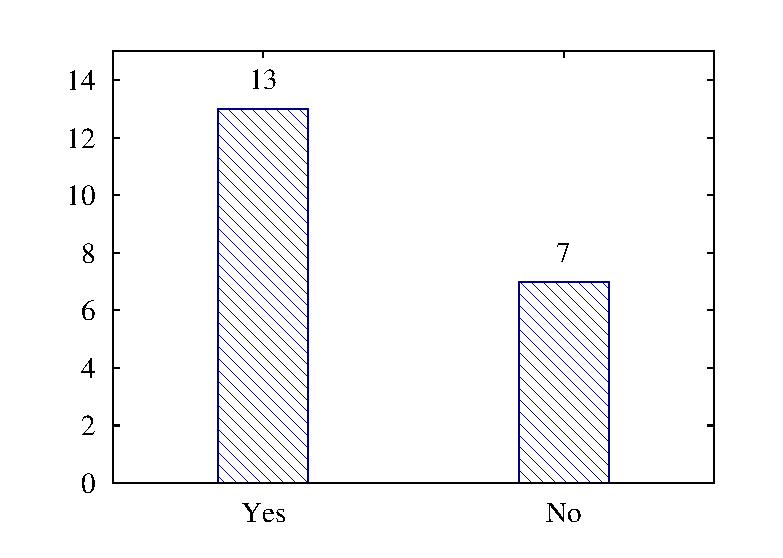
\includegraphics[scale=.7]{files/question1/question1.eps}
\caption{Participants satisfaction with the login methods used in apps.}
\label{fig:digraph}
\end{figure}

\subsection{Participants Opinion on Conventional Login}
Most of the participants found the authentication method to be normal (45\%) or even hard (34\%) for them as seen on the Figure 5.5, implying to the size of the keyboard on the device. Similar results applied to the question of, whether they were annoyed by the process, shown at Figure 5.6. Given the answers values of 1 to 3, 1 being ''Easy/Low'', the average to both of these questing would be 2.15. 

As seen from the Figures 5.7 and 5.8, the conventional login method would push users away from the application or make them change their passwords to something easier to type. 35\% of the participants would definitely use the application less and 30\% are considering it, making the application less appealing to 65\% of users because of the authentication process. This method is also pushing 70\% of the  users to change their passwords, making them more vulnerable to intruders.  

This shows how damaging the conventional method could be for the user base and reputation of the application. Also users are put to danger by allowing themselves to use weaker passwords.

\begin{figure}[H]
\centering
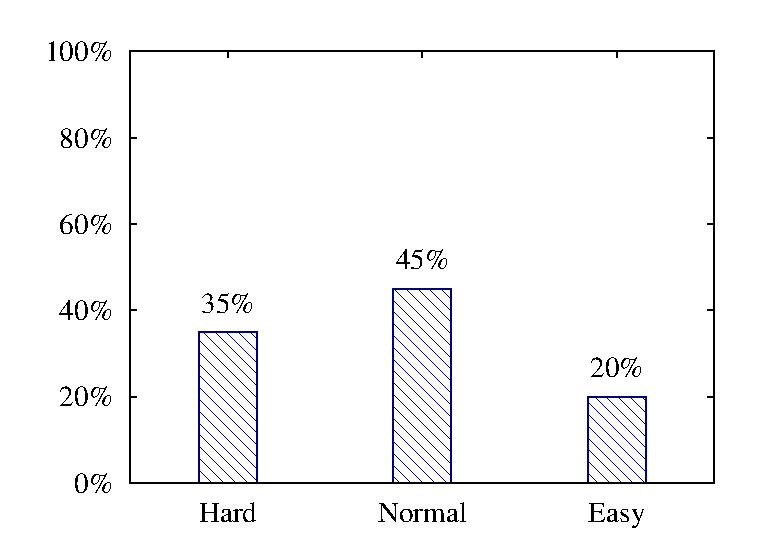
\includegraphics[scale=.7]{files/question3/question3.eps}
\caption{Complexity in the authentication process with conventional method.}
\label{fig:digraph}
\end{figure}

\begin{figure}[H]
\centering
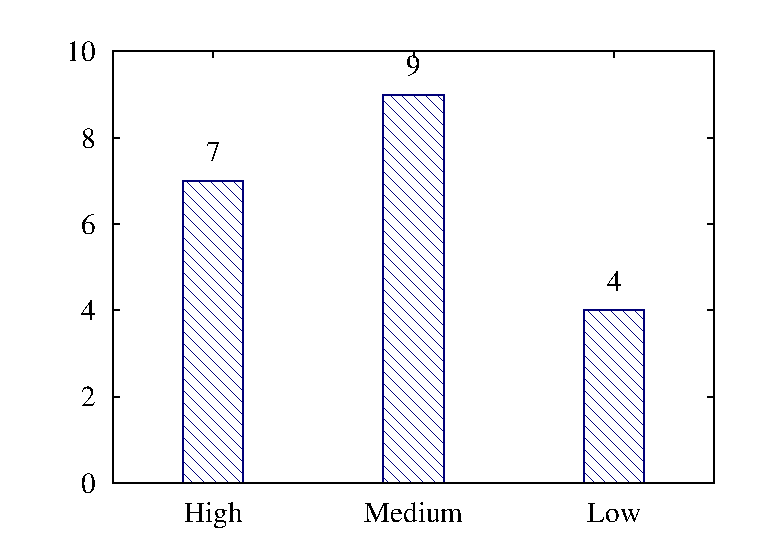
\includegraphics[scale=.7]{files/question4/question4.eps}
\caption{Level of annoyance caused by conventional method.}
\label{fig:digraph}
\end{figure}

\begin{figure}[H]
\centering
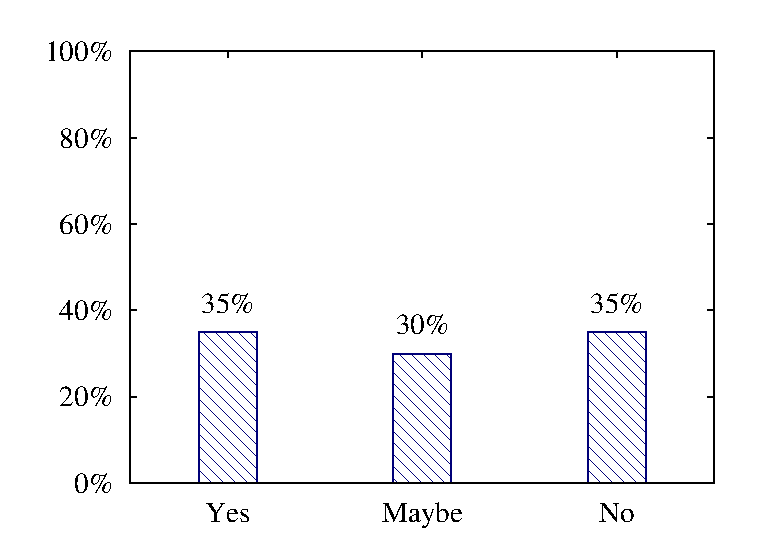
\includegraphics[scale=.7]{files/question5/question5.eps}
\caption{Participants being pushed away by the inconvenience.}
\label{fig:digraph}
\end{figure}

\begin{figure}[H]
\centering
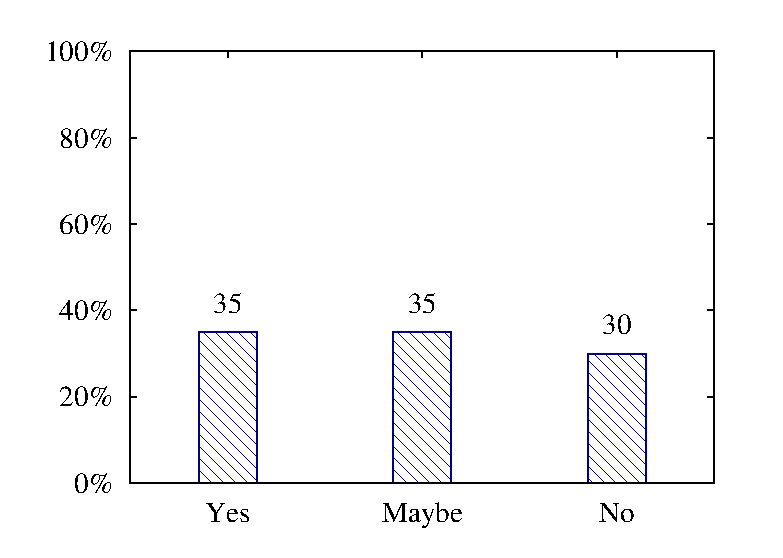
\includegraphics[scale=.7]{files/question6/question6.eps}
\caption{Discomfort making users change their passwords. }
\label{fig:digraph}
\end{figure}

\subsection{Participants Opinion on the Proposed Solution}

The participants were using this method for the first time and were asked questions about the simplicity of it, to see whether this solution could be justified. 

Compared to the conventional method, the proposed solution seems to be easier to use, see the Figure 5.9. Nobody thought it was hard. 75\% of the participants found the method easy and 25\% normal. Given the answers values of 1 to 3, 1 being ''Easy'', the average would be 1.25. This is also reflected on usage of the application, where nobody answered they would definitely use the application less, shown on Figure 5.10, because of the provided method. Only 15\% of participants would consider using it less. 

The given method was composed of two steps. Before authenticating themselves, they had to register their credentials with the application. 75\% of the participants found the process easy and nobody felt confused, as seen on Figure 5.11. When asked to change the password or pattern saved in the application, some participants felt confused in the process - 25\%, but 55\% found it intuitive, as seen in Figure 5.12.

\begin{figure}[H]
\centering
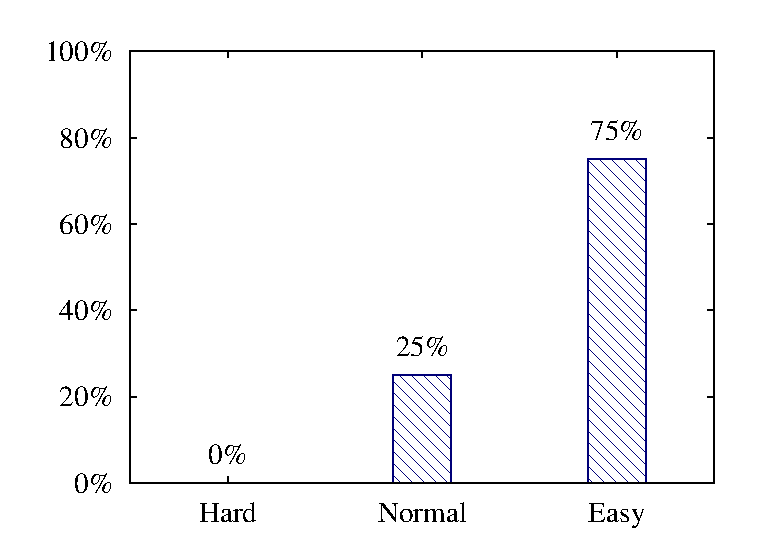
\includegraphics[scale=.7]{files/question7/question7.eps}
\caption{Complexity in the authentication process with pattern based method.}
\label{fig:digraph}
\end{figure}

\begin{figure}[H]
\centering
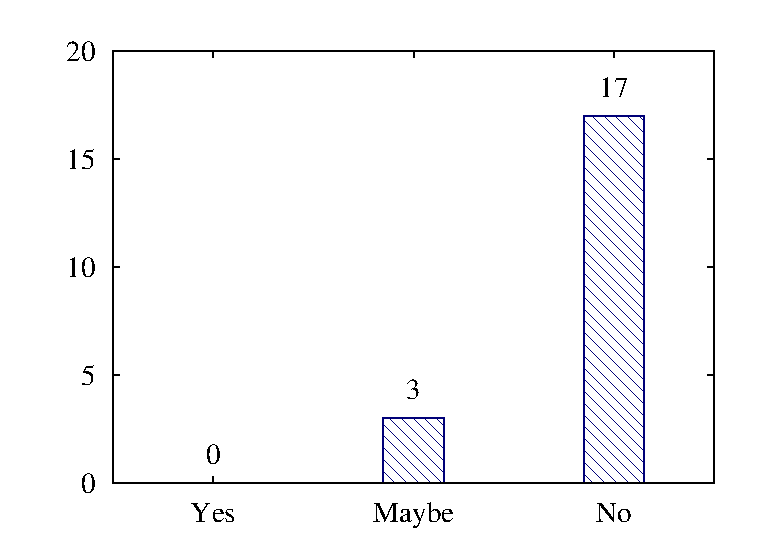
\includegraphics[scale=.7]{files/question8/question8.eps}
\caption{Participants being pushed away by the discomfort.}
\label{fig:digraph}
\end{figure}

\begin{figure}[H]
\centering
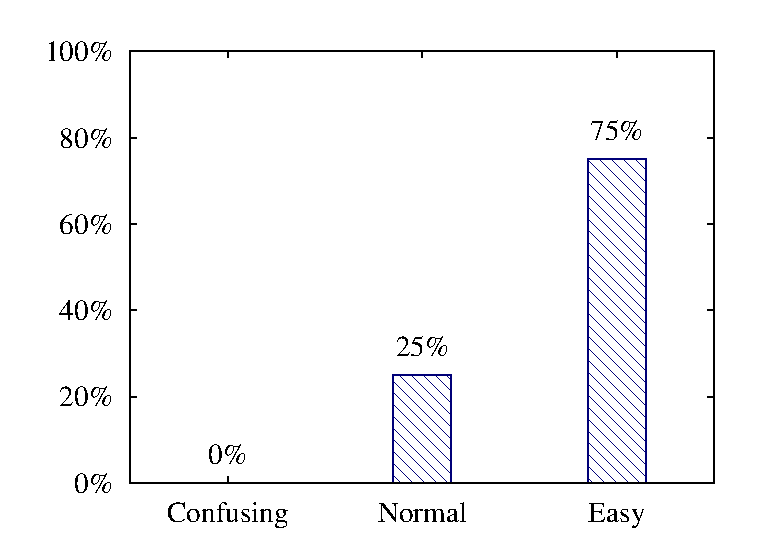
\includegraphics[scale=.7]{files/question9/question9.eps}
\caption{Simplicity of the credentials saving process.}
\label{fig:digraph}
\end{figure}

\begin{figure}[H]
\centering
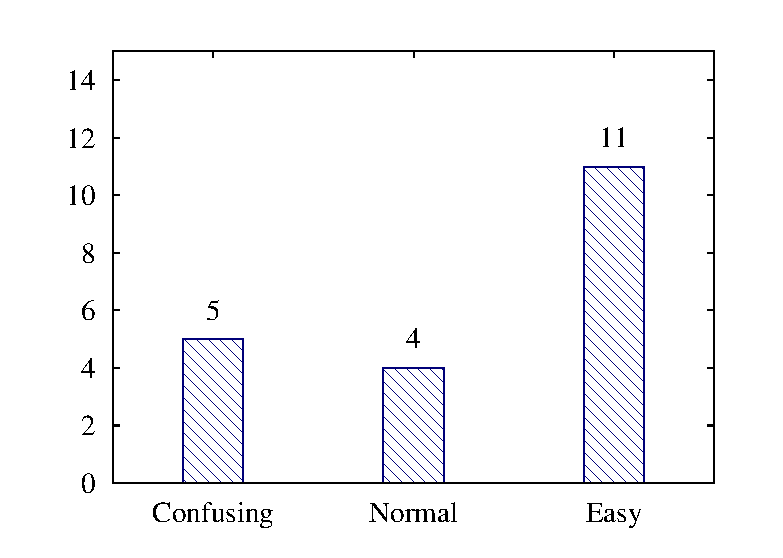
\includegraphics[scale=.7]{files/question10/question10.eps}
\caption{Simplicity of the password or pattern changing process.}
\label{fig:digraph}
\end{figure}

\section{Summary}
In this chapter the usability of the proposed mechanism is validated.  With the conventional model, 35\% of the participants found it hard and annoying. 65\% of participants felt the process to be repulsive and 70\% sensed the need to change their passwords to something easier to type, therefore less secure. Opposed to the conventional method, the proposed solution was easier to the user, as 75\% of the participants found it easy to use and therefore they were not losing interest in the application, as only 15\% found it slightly repulsive. To store credentials, users have register their credentials and sometimes change their passwords. Although these are additional steps in the process, most participants find them easy to complete.



% ---------------------------------------------------------------------------
%: ----------------------- end of thesis sub-document ------------------------
% ---------------------------------------------------------------------------

